% Copyright (c) 2017-2019 Michael C. Heiber
% This file is part of the Excimontec project, which is subject to the MIT License.
% For more information, see the LICENSE file that accompanies this software.
% The Excimontec project can be found on Github at https://github.com/MikeHeiber/Excimontec

\documentclass[%
 reprint,onecolumn,notitlepage,
superscriptaddress,longbibliography,
 amsmath,amssymb,
 aps,rmp,floatfix,
]{revtex4-1}
\bibliographystyle{unsrtnat}
\setcitestyle{numbers,square}

\usepackage[margin=1in]{geometry}
\usepackage[utf8]{inputenc}
\usepackage{amsmath}
\usepackage{hyperref}
\usepackage{minted}
\usepackage[version=4]{mhchem}

\begin{document}

\title{Excimontec v1.0 User Manual}
\author{Michael C. Heiber}

\date{\today}

\maketitle

\tableofcontents

\newpage

\section{Introduction}

Kinetic Monte Carlo simulations are a powerful computational tool that have been used in concert with experiments and more detailed theoretical methods to understand and optimize organic semiconductor materials and devices.\cite{heiber2019chapter} 
However, despite over 30 years of applying KMC tools to organic semiconductors, no widespread or standardized software tools have taken hold in the community. 
Instead, many research groups around the world have maintained private codebases of varying complexity, efficiency, and reliability. 
As a result, there have been large barriers to entry for new researchers and a lot of repeated effort throughout the community that would be much better off applied to pushing the capabilities of the technique and further refining the physical models.

Excimontec represents an honest effort to bring the community together around a well-tested, optimized, reliable, and accessible open-source tool for performing KMC simulations of organic electronic devices. 
The current version (v1.0) implements a cubic lattice-based model for the organic semiconductor layer and is focused on simulation tests for neat single carrier diodes and binary donor-acceptor organic photovoltaic devices.
Future extension of the software to simulate light emitting diodes and field-effect transistors is planned.
The software is written in modern C++ and is optimized for efficient pleasingly parallel execution on high performance computing clusters using MPI. 
This software package uses object-oriented design and extends the KMC\_Lattice framework.\cite{heiber2019joss} 
It is also designed to work with the Ising\_OPV software tool for creating and importing bulk heterojunction morphologies.\cite{heiber2018joss}

\section{Simulation Tests}

Excimontec is designed to allow users to select and run a particular simulation test with a specific set of input parameters.
Currently there are five different simulations tests available:
\begin{enumerate}
    \item Exciton Diffusion Test
    \item Time-of-Flight Charge Transport Test
    \item Internal Quantum Efficiency Test
    \item Dynamics Test
    \item Steady State Charge Transport Test
\end{enumerate}
Choice of a particular test and the input parameters is made within the parameter file that is then passed as an input argument to the program.
An example parameter file (parameters\_default.txt) is provided in the root repository directory to be used as a starting point for customization.
A valid parameter file has strict formatting rules, so users should simply copy the default parameter file and then modify the values as needed.
The program should generate an error message if you accidentally mess up the formatting or enter an invalid value for any of the parameters.

Below, the basics of each simulation test are explained and several examples of the types of physical phenomena that can be simulated are provided.
If you have further questions about the capabilities and options for any of the simulation tests, please post a question in \href{https://github.com/MikeHeiber/Excimontec/issues}{Issues section} on the Github website.

\subsection{Exciton Diffusion Test}

This simulation mode is selected by turning on the Enable\_exciton\_diffusion\_test option and is designed to allow users to test exciton diffusion behavior under a variety of different conditions.
The simulation is performed by randomly placing excitons one at a time on the lattice, letting them diffuse via their normal hopping mechanism, and finally recording the displacement distance upon exciton recombination back to the ground state.
The simulation is performed independently on each processor core until the number of tested excitons reaches the specified N\_tests value from the parameter file.
The independent results from each processor are then aggregated and the mean and standard deviation of the exciton diffusion length are calculated and output to the analysis\_summary file.

When performed on a neat material, one can determine how properties like energetic disorder, temperature, exciton hopping rate, and exciton lifetime affect the diffusion length.
For example, Fig. \ref{fig:exciton_diffusion_example}(a) shows how the exciton diffusion length increases as the singlet exciton hopping rate prefactor increases in a neat material with an uncorrelated Gaussian density of states.
Then, Fig. \ref{fig:exciton_diffusion_example}(b) shows how the exciton diffusion length decreases as the energetic disorder increases and slows down the diffusion process.
These types of simulations are a good way to determine the materials parameters required to reach a desired exciton diffusion length or to probe more fundamental diffusion phenomena.

\begin{figure}[h]
    \centering
    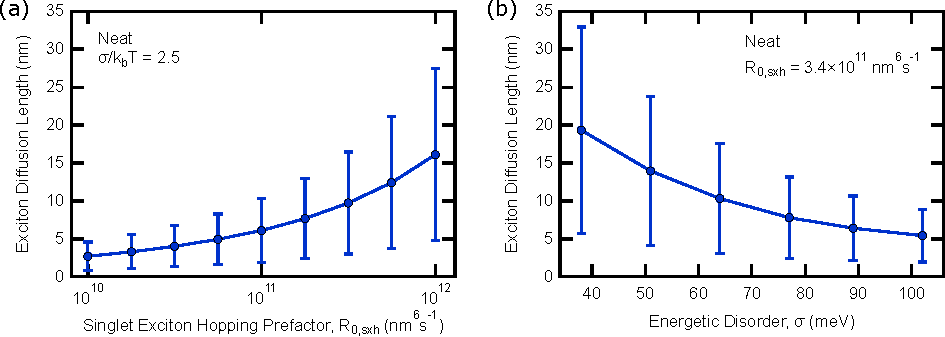
\includegraphics{Exciton_diffusion_example_data.pdf}
    \caption{Exciton diffusion test data showing how the exciton diffusion length depends on (a) the exciton hopping rate prefactor and (b) the energetic disorder of the material. Error bars show the first standard deviation of the diffusion length data.}
    \label{fig:exciton_diffusion_example}
\end{figure}

\subsection{Time-of-Flight Charge Transport Test}

This simulation mode is designed to produce an ideal time-of-flight (ToF) charge transport experiment.
In the ToF experiment, a very thin sheet of charge carriers is generated at one surface of film by a laser pulse, and then the transient current response is measured as the charge carriers move through the film and are eventually extracted at the opposite electrode.
ToF experiments have been widely used to probe the fundamental charge transport behavior of organic semiconductors as a function of electric field, temperature, charge carrier density, etc.\cite{baessler1993pssb}
Whereas the experiment is limited in that information can only be extracted from analysis of the current transient, KMC simulations of the same test can provide much more detailed information.

To perform this test, one must turn on the Enable\_ToF\_test option.
The ToF test simulates the transport of an ultrathin sheet of charge carriers (electrons or holes) through the lattice.
The number of charge carriers in the sheet is set by the ToF\_initial\_polarons parameter, and they hop through the lattice under the influence of the defined Internal\_potential until they are extracted at the opposite side.
The transit time of each extracted charge carrier is recorded, and any charge carriers stuck in the lattice longer than the specified ToF\_transient\_end cutoff time are removed from lattice and not included in the collection of transit times.
The process is repeated until the total number of carriers simulated equals the N\_tests parameter.
The simulation is performed independently on each processor, and the results are aggregated and averaged at the end.
In addition to an average transit time and mobility, the simulation provides the current density transient, charge carrier density transient, average occupation energy transient, average mobility transient, and transit time probability histogram.
Examples of these results are provided in Fig. \ref{fig:tof_example}.

\begin{figure}[h] % 16.5 cm column width
    \centering
    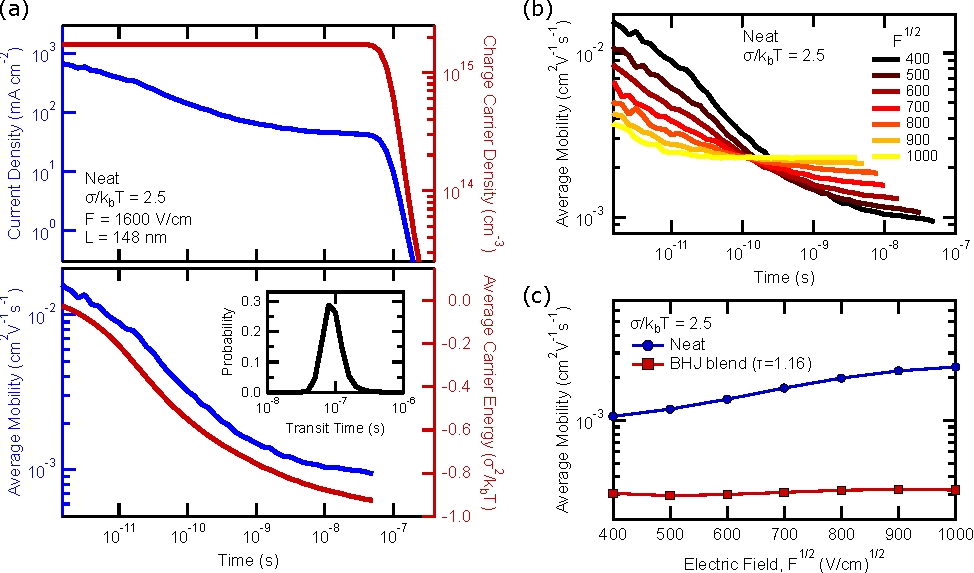
\includegraphics{ToF_example_data.pdf}
    \caption{Time-of-flight charge transport test results showing (a) neat material transients with transit time distribution inset, (b) neat material electric-field-dependent mobility relaxation, and (c) electric-field-dependent mobility in a neat material and a bulk heterojunction blend.}
    \label{fig:tof_example}
\end{figure}

The ToF charge transport test provides users with a detailed tool to probe the transient mobility relaxation phenomena and how it is affected by the density of states, temperature, electric field, charge carrier density, material morphology, etc. 
For a neat material, Fig.\ \ref{fig:tof_example}(a) shows relaxation of the current density and average mobility due to charge carrier thermalization into the tail of the DOS until reaching nondispersive, steady state transport after approximately 10 ns.
Figure \ref{fig:tof_example}(b) shows the how the transition from dispersive to nondispersive transport shifts with electric field in a neat material and how the steady state mobility increases as the electric field increases. 
Figure \ref{fig:tof_example}(c) demonstrates how the electric-field dependence of mobility can also be quantified in bulk heterojunction blends to determine the complex interplay between energetic disorder ($\sigma$) and domain network tortuosity ($\tau$) as shown previously.\cite{heiber2017prapp2}

As more advanced features, users can also create the initial charge carriers at a specific energy position within the density of states instead of randomly populating it to probe how the starting energy of the charge carriers affects the transient behavior.
To do this, one must turn off the Enable\_ToF\_random\_placement option, turn on the Enable\_ToF\_energy\_placement option, and set the ToF\_placement\_energy.
In addition, one can produce charge extraction maps to probe for fluctuations in current density across the area of the film that may arise due to energetic fluctuations from the correlated disorder model or morphological features in a bulk heterojunction film by turning on the Enable\_extraction\_map\_output option.

\subsection{Internal Quantum Efficiency Test}

The internal quantum efficiency (IQE) test allows users to simulate a common photovoltaic device characterization technique.
It is a steady state measurement that quantifies the fraction of absorbed photons that are successfully converted into extracted charge carriers. 
The measurement is commonly done under short-circuit conditions, but one can also apply a bias.
The Excimontec IQE test additionally provides a detailed breakdown of the various loss mechanisms that produce the final IQE value, including the exciton dissociation yield, the charge separation yield, and the bimolecular recombination loss fraction.

The IQE test is selected by turning on the Enable\_IQE\_test option and proceeds by randomly creating excitons on donor or acceptor sites at a rate specified by the Exciton\_generation\_rate parameter of each material.
Exciton generation stops once the number of excitons created equals the N\_tests parameter.
The simulation finishes once all charge carriers are extracted from the lattice or once the IQE\_time\_cutoff is reached.
The simulation is performed independently on each processor, and the results are aggregated and averaged at the end.

Figure \ref{fig:IQE_example} provides some examples for how the IQE test can be used. Figure \ref{fig:IQE_example}(a) shows the exciton dissociation yield in a donor-acceptor bulk heterojunction blend with a domain size of 16 nm and demonstrates how the yield increases as the exciton hopping rate increases. 
Since these parameters were also tested using the exciton diffusion test, the increase in dissociation yield can also be related to the corresponding increase in the exciton diffusion length.
The IQE test can also be used to probe charge separation phenomena and reproduce behavior that has been widely studied in the literature.\cite{heiber2019chapter}
For example, Figure \ref{fig:IQE_example}(b) shows the electric-field dependence of the charge separation yield for a donor-acceptor bilayer architecture with different degrees of polaron delocalization, following previously observed trends.\cite{deibel2009prl}
One can also explore many other dependencies such as temperature, energetic disorder, charge hopping rates, or various morphological features using a bulk heterojunction architecture.

\begin{figure}[h]
    \centering
    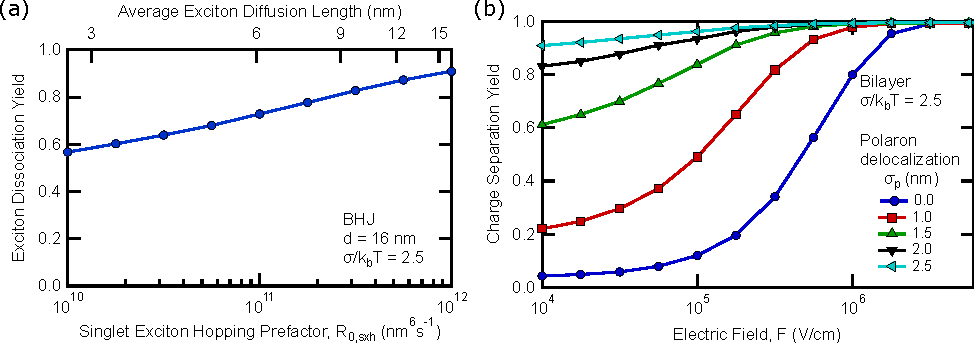
\includegraphics{IQE_example_data.pdf}
    \caption{Internal quantum efficiency test results showing (a) exciton dissociation yield in a donor-acceptor bulk heterojunction morphology and (b) charge separation yield in a donor-acceptor bilayer device architecture.}
    \label{fig:IQE_example}
\end{figure}

\subsection{Dynamics Test}

Another popular type of experiment is a pump-probe experiment, where a laser pulse (pump) creates an initial population of excitons in the film that then evolves over time.
Experimentally, the probe can be electrical or optical, but ideally one would like to measure how the populations of the different excited states evolve over time to determine the kinetics of the various mechanisms.
The Excimontec dynamics test provides a wide variety of information about how the singlet exciton, triplet exciton, electron, and hole populations change over time.

The dynamics test is selected by turning on the Enable\_dynamics\_test option and begins by creating the initial excitons randomly throughout the lattice until reaching the concentration specified by the Dynamics\_initial\_exciton\_conc parameter.
The excitons are then allowed to diffuse, dissociate, or recombine as they will, and the simulation is terminated once all of the excitons and charge carriers have disappeared from the lattice or once the Dynamics\_transient\_end cutoff time has been reached.
The cycle is then repeated until the total number of excitons tested equals the N\_tests parameter.
The simulation is performed independently on each processor, and the results are aggregated and averaged at the end.

Figure \ref{fig:dynamics_example} shows several examples of results from dynamics tests performed on a donor-acceptor bulk heterojunction blend.
Figure \ref{fig:dynamics_example}(a) shows how an initial population of singlet excitons diffuses and relaxes into the tail of the DOS and mostly dissociates to form polarons (electrons and holes).
This example also shows a small population of triplet excitons forming due to intersystem crossing from the singlet to triplet excitonic states.
The polaron population then also relaxes into the tail of the DOS and decays at several timescales due to competing charge recombination mechanisms, with geminate recombination starting at the 1 ns timescale and bimolecular recombination starting at the 1 $\mu$s timescale.
Figure \ref{fig:dynamics_example}(b) focuses on singlet exciton dissociation dynamics, showing how exciton dissociation occurs faster when the exciton hop rate increases.
Figure \ref{fig:dynamics_example}(c) focuses on charge carrier recombination dynamics showing how increasing polaron delocalization reduces the amount of geminate recombination and slows down the bimolecular recombination process.
The dynamics test is particularly powerful for investigating how domain size and mobility together cause deviation from the Langevin model for encounter-limited bimolecular recombination.\cite{heiber2015prl,heiber2016prb}
It can also be used to probe the impact of energetic disorder, density of states shape, and the charge-transfer state lifetime on the bimolecular recombination rate and recombination order.\cite{coropceanu2017jpcc}

\begin{figure}[h]
    \centering
    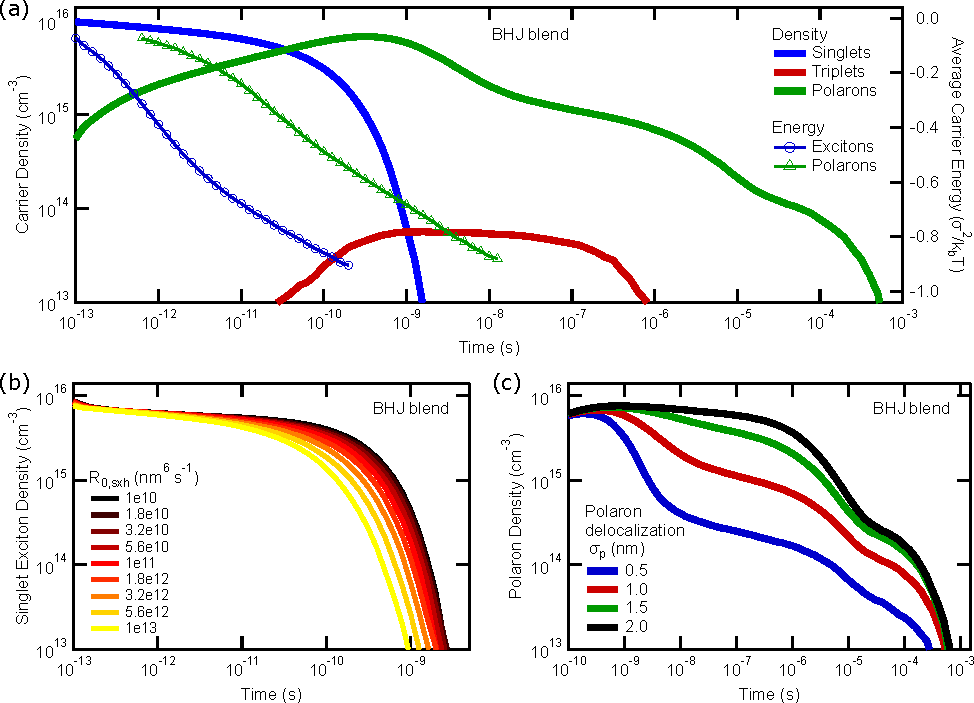
\includegraphics{Dynamics_example_data.pdf}
    \caption{Dynamics test results showing (a) full carrier density and energy transients, (b) exciton dissociation dynamics, and (c) charge carrier recombination dynamics in a BHJ blend.}
    \label{fig:dynamics_example}
\end{figure}

\subsection{Steady State Charge Transport Test}

While the time of flight charge transport test is a good way to study transient effects such as mobility relaxation, one may also want to focus on steady state quasi-equilibrium transport behavior that can be relevant for different applications.
The steady state transport test is designed to probe hole transport in a neat donor material or in donor-acceptor blends.
Transport in doped semiconductors can also be simulated using the custom density of states import feature.

The test begins by creating holes randomly on donor sites until reaching the Steady\_carrier\_density value defined in the parameter file.
The simulation then enters the equilibration phase where holes are allowed to undergo hopping events under the applied bias specified by the Internal\_potential parameter until the number of executed events equals the N\_equilibration\_events parameter value.
The simulation then enters the measurement phase and holes continue hopping until the number of events executed in the measurement phase equals the N\_tests parameter.
Periodic z-direction boundaries must be used and allow charge carriers to continue hoping indefinitely under the applied bias.

In addition to the state state mobility, this test calculates the transport energy and equilibration energy. 
It also provides detailed information about the density of states (DOS) and the density of occupied states (DOOS) under the given simulation conditions.
The DOS and DOOS are both calculated with and without including electrostatic interactions to show how the state energies are modified by the presence of the charge carriers.
The ratio of the DOOS to the DOS can then be fit to the Fermi-Dirac function to determine the Fermi energy and the effective temperature, and the Fermi energy can be combined with the transport energy to determine the Seebeck coefficient.\cite{zuo2019aem}

Fig.\ \ref{fig:steady_transport_example} shows example data for steady state charge transport of holes traveling through a neat material with a Gaussian density of states ($\sigma / k_\text{b}T = 2.5$) and $p = 1 \times 10^{16}$ cm$^{-3}$.
As expected, this example shows electric-field activated mobility that roughly follows the Poole-Frenkel model ($\ln\mu\propto F^{1/2}$).
In addition, at low electric-field, the calculated equilibration energy is very close to the true equilibration energy that resides at $-\sigma^2 / k_\text{b}T$ relative to the average site energy. 
The electric field perturbs the carriers so that they sit at higher energies than they would under true zero-field equilibrium conditions.
At higher electric field, the DOOS shifts to higher energy and the equilibration energy also increases in an analogous fashion to the effect of an increase in temperature, as expected from the effective temperature model.\cite{baranovskii2014pssb}
Another interesting feature captured here is the appearance of a high energy shoulder in DOS due to the electrostatic interactions between charge carriers.
When the system is occupied with carriers at $p = 1 \times 10^{16}$ cm$^{-3}$, the DOS does not have simple Gaussian shape.
Sites near existing charge carriers have energies that are significantly shifted upward due to electrostatic repulsion.
The steady state charge transport test allows users to probe the complex impacts of electric field, carrier density, temperature, density of states, and even morphology on the steady state bulk charge carrier mobility that can then be compared with experimental results. 

\begin{figure}[h]
    \centering
    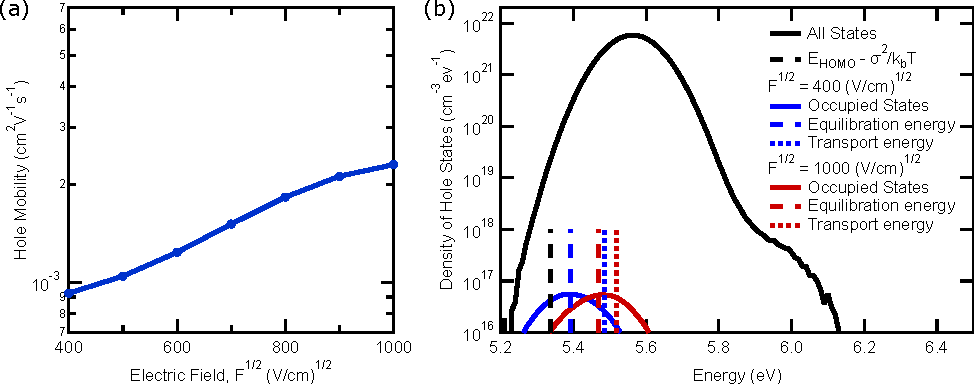
\includegraphics{Steady_transport_example_data.pdf}
    \caption{Steady state charge transport test results showing (a) electric-field dependent mobility and (b) density of states data for hole transport using a Gaussian density of states ($\sigma / k_\text{b}T = 2.5$) and $p = 1 \times 10^{16}$ cm$^{-3}$.}
    \label{fig:steady_transport_example}
\end{figure}

\section{Simulation Parameters and Model Details}

Specifying which simulation test to run, which device architecture to simulate on, which mechanism models to use, and all of the electronic materials properties and parameters is done using the parameter file.
A single parameter file is used to run the KMC simulation test for a single set of parameters.
To do parameter sweeps, one must create separate parameter files for each condition and then run separate simulations for each.
While this can be tedious when manually creating and modifying the parameter files, shell scripts can be used to quickly create a series of parameter files for a parameter sweep, and simulation job arrays can be used to submit all of the simulations in a parameter sweep and group the individual simulations together.
This part of the user manual will go through each section of the parameter file and explain what each input parameter is used for.

\subsection{KMC Algorithm Parameters}\label{sub:KMC_algorithms}

At any given time, there are a number of different mechanisms that can occur in an organic semiconductor device under operational conditions. 
Excitons and polarons can move, dissociate, recombine, etc. 
In a KMC simulation, each time the state of the system changes in any way, we say that an event has occurred. The goal of a KMC simulation is to simulate the evolution of the system over time, one event at a time, to determine the transient behavior or to gather statistics about the steady state behavior.

\subsubsection{First-reaction Method:}

Here, the formalism of the Gillespie first reaction method (FRM) is implemented to determine which event will occur next.\cite{gillespie1976jcp} 
In a system containing numerous excitons and polarons, there are a number of different possible events that can occur at any given time. 
To determine when each will occur, the wait time for each possible event is calculated,
$$t = \frac{-\ln{X}}{R},$$
where $X$ is a random number between 0 and 1 chosen from a uniform distribution and $R$ is the rate of the particular event. 
Excimontec uses the Mersenne twister pseudorandom number generator implemented in the C++ 11 standard library for high quality random number generation.
With the wait time calculated for all possible events, the event with the shortest wait time is executed. 
An extension of this method is the assumption that the majority of excitons and polarons are independent and that the calculated events can be put into a sorted schedule queue to be executed one by one as their scheduled time comes. 
After each iteration, only a small number of newly disabled events must be removed from the queue and only a small number of newly enabled events must be calculated and added to the queue. 
As a result, all possible events do not need to be recalculated after each iteration.

\subsubsection{BKL Algorithm:}

One also does not need to store all possible events for each exciton or polaron since only one of them will be executed before calculating the next event for that exciton or polaron. 
To efficiently determine the chosen event among many possibilities for a single exciton or polaron, the Bortz-Kalos-Lebowitz algorithm is used.\cite{bortz1974prb}
Instead of drawing a random number to calculate the wait time for each possible mechanism, the event can be chosen with only a single random number. 
One first calculates the rates for all possible ($N$) events, places them in an array, and adds them up,
$$R_\text{sum} = \sum_{i=0}^N R_i$$
One then generates a single random number and then finds the smallest event index ($i=n$) such that,
$$\sum_{i=0}^n R_i > R_\text{sum}X.$$
The $n^\text{th}$ event becomes the selected event, and the wait time for the event is calculated using $R_\text{sum}$. 
With the BKL algorithm, the event queue remains relatively small since only one event is queued per exciton or polaron in the simulation.

\subsubsection{Event Recalculation}

However, polarons specifically have long-range electrostatic interactions with each other, and their events are not truly independent from each other.
The motion of one or several polarons modifies the electrostatic potential landscape, which should have an impact on the next event of other nearby polarons. 
When using the first-reaction method, this effect is ignored to save computing time. 
If one wants to check the significance of this simplifying assumption, the full recalculation algorithm is also implemented and can be enabled in the parameter file. 
With the full recalculation method, all events for all excitons and polarons are recalculated after each iteration of the simulation, thereby ensuring that the next event takes into full consideration all changes to the system.

As an alternative, a selective recalculation method is also implemented that allows users to selectively update the events of all objects near the previous event within a user defined recalculation cutoff radius ($r_\text{recalc}$).\cite{heiber2012jcp} 
By choosing the optimal recalculation cutoff radius in the parameter file, users can ensure that there is minimal impact from the simplifying assumptions of the first-reaction method, while also saving considerable computational time relative to the full recalculation method.

\subsection{Lattice Parameters}

The simulation volume is a cuboid shape and users must identify the dimension in the x, y, and z dimensions, which are the length ($L$), width ($W$), and height ($H$), respectively.
In addition to the lattice size, users can set boundary conditions as either hard boundaries or periodic boundaries. 
In all of the simulation tests, the z-direction is treated as the charge transport direction and hard z-direction boundaries can represent the electrodes or material surface/interface. 
Periodic boundaries will often be desired in the x- and y-directions to simulate a thin film, but users can apply hard boundaries to investigate transport confinement effects.
Users must also set the lattice unit size ($a$), which determines the real space distance between sites on the lattice and the total density of states.
Another important general property of the lattice determine here is the temperature ($T$).
Finally, the internal potential parameter ($V_\text{int}$) determines the voltage drop across the height (z-direction) of the lattice and is used to control the electric field in the simulation. 

\subsection{Device Architecture Parameters}

Users can choose from a number of difference device architectures for the simulation box.
One can implement a single neat material simulation that takes on the specified donor materials properties.
One can create a donor-acceptor bilayer structure and specify the thickness of each sub-layer.
One can use a random donor-acceptor blend in which sites in the lattice are randomly assigned as acceptor sites until reaching the specified acceptor concentration.
Instead of using one of these simple built-in device architecture models, users can also import donor-acceptor morphologies as a single morphology that will be used for all simulations or a set of morphologies that will randomly assigned to each simulation. 
In particular, the morphology import feature is designed to allow users to import bulk heterojunction morphologies created using the Ising\_OPV simulation tool.\cite{heiber2018joss}
However, any morphology conforming to the Ising\_OPV morphology file format can be imported.

\subsection{Exciton Mechanisms and Parameters}

Here, we describe each of the exciton mechanisms currently implemented and their associated parameters.
For most parameters, the parameter file allows users to specify different values for the donor and acceptor sites even though explicitly defined separate variables for each are not shown below.

\subsubsection{Exciton Generation}

To simulate the creation of optically generated excitons, singlet excitons are created randomly on donor or acceptor sites based on the generation rates specified in the parameter file. 
Currently, the exciton generation model does not include any interference effects or extinction effects that can cause generation rate gradients in real devices. As a result, generation rates are uniform in the thickness direction, which is a reasonable first-order approximation for thin films ($\approx$100~nm) on a non-reflecting substrate. 
For calculating the singlet exciton generation rate,
$$R_\text{sxg} = G V.$$
where, $G$ is the exciton generation rate of the material and $V$ is the total volume of the material in the lattice.
It is assumed that no triplet excitons are generated by illumination due to the fact that it is a spin forbidden transition,
$$R_\text{txg} = 0.$$

\subsubsection{Exciton Hopping}

Transport of excitons from site to site can occur by two different mechanisms, F{\"o}rster resonance energy transfer (FRET)\cite{forster1948} or Dexter electron exchange.\cite{dexter1953jcp} 
Under different conditions, one of the two mechanisms usually dominates, so both mechanisms do not need to be calculated for every iteration of the simulation. 
Singlet excitons are generated optically and can also readily emit a photon. 
Due to this property, singlet excitons can move from site to site by emitting and then absorbing a virtual photon, and this longer-range process typically dominates over the Dexter electron exchange mechanism. 
Conversely, triplet excitons have spin forbidden optical transitions, thereby making photon emission and absorption very slow processes. 
As a result, the energy transfer mechanism is negligible, and the shorter-range Dexter electron exchange mechanism dominates. 
With Dexter electron exchange, electrons on neighboring sites are exchanged via a charge transfer mechanism. 
The excited electron moves to a neighboring site, and the exciton effectively moves.

Regardless of the mechanism, hopping events are calculated for all destination sites within the FRET cutoff radius, $r_{\text{FRET,cut}}$, and the driving force of the transition is based on the initial and final state energies.
For singlet excitons, the state energy is defined
$$E_{\text{s}} = E_\text{HOMO} - E_\text{LUMO} - E_\text{B}$$
where $E_\text{HOMO}$ is the highest occupied orbital energy, $E_\text{LUMO}$ is the lowest unoccupied orbital energy, and $E_\text{B}$ is the exciton binding energy.
For triplet excitons, 
$$E_{\text{t}} = E_\text{s} - \Delta E_\text{ST}$$
where $\Delta E_\text{ST}$ is the singlet-triplet splitting energy.

\subsubsection*{\textbf{F{\"o}rster resonance energy transfer (FRET) model:}}

The rate for FRET-based singlet exciton hopping is defined
$$R_{\text{sxh,FRET},ij} = R_{0,\text{sxh}} \left( \frac{1}{d_{ij}} \right)^6 f_\text{B} \left( \Delta E_{\text{FRET},ij}\right),$$
where $R_{0,\text{sxh}}$ is the singlet exciton hopping prefactor, $d_{ij}$ is the distance between sites, and
$$\Delta E_{\text{FRET},ij} = E_{\text{s},j} - E_{\text{s},i}.$$
$f_\text{B}$ is the Boltzmann function,
$$f_\text{B} \left( \Delta E_{ij}\right) = \begin{cases}
\exp{\left( \frac{-\Delta E_{ij}}{k_\text{B} T} \right)} & \Delta E_{ij} > 0 \\
1 & \Delta E_{ij} \le 0 \\
\end{cases}$$
where $k_\text{B}$ is the Boltzmann constant and $T$ is the temperature.

\subsubsection*{\textbf{Dexter electron exchange model:}}

The rate for Dexter-based exciton hopping is defined
$$R_{\text{txh,Dex},ij} = R_{0,\text{txh}} \exp{\left(- 2 \gamma_{\text{t}} d_{ij} \right)} f_\text{B} \left( \Delta E_{\text{Dex},ij}\right),$$
where $R_{0,\text{txh}}$ is the triplet exciton hopping prefactor, $\gamma_{\text{t}}$ is the triplet localization parameter, and
$$\Delta E_{\text{Dex},ij} = E_{\text{t},j} - E_{\text{t},i}.$$

\subsubsection{Exciton Dissociation}

Exciton dissociation is essentially a transition from an exciton state to a charge-transfer (CT) state that spans a donor-acceptor interface. 
The event proceeds by a charge transfer mechanism. 
For an exciton located on a donor site, an electron transfers from the donor site to an acceptor site. 
For an exciton located on an acceptor site, a hole transfers from the acceptor site to a donor site. 
As a result, the mechanism is simulated using a charge transfer model. 
Excimontec implements two options for charge transfer models, the Miller-Abrahams phonon-assisted tunneling model\cite{miller1960pr} and a simplified Marcus model \cite{marcus1956jcp} that implements a polaronic mechanism.

Regardless of the model used, dissociation events are calculated for all nearby destination sites within the exciton dissociation cutoff radius, $r_{\text{xd,cut}}$, and the driving force for this transition depends on the energies of the initial final states. For singlet excitons,
$$\Delta E_{\text{sxd},ij} = E_{\text{CT},ij} - E_{\text{s},i},$$
and for triplet excitons,
$$\Delta E_{\text{txd},ij} = E_{\text{CT},ij} - E_{\text{t},i},$$
where $E_{\text{CT},ij}$ is the CT state energy. 
For the dissociation of an exciton starting from a donor site, 
$$E_{\text{CT},ij} = E_{\text{HOMO}_\text{D},i} - E_{\text{LUMO}_\text{A},j} + E_\text{B,CT} \left( d_{ij} \right) + E_\text{C}(q_i) + E_\text{C}(q_j) - e \mathbf{d}_{ij} \cdot \mathbf{F},$$
where $E_\text{B,CT}$ is the CT state binding energy, $E_\text{C}(q)$ is the electrostatic interaction energy term for the newly formed polarons interacting with all other polarons in the system, $e$ is the elementary charge constant, $\mathbf{d}_{ij}$ is the CT state dipole displacement vector, and $\mathbf{F}$ is the internal electric field vector.
An analogous expression is used for dissociation of an an acceptor exciton.
It is worth noting here that the different spin states of a CT state are not modeled here, and CT states with singlet or triplet spin are treated as the same and therefore assumed to have the same energies and the same mechanism rates. 
Moving on, the CT state binding energy is defined
$$E_\text{B,CT} \left( d_{ij} \right) = \frac{-e^2}{4 \pi \epsilon \epsilon_0 d_{ij}},$$
where $\epsilon$ is the dielectric constant and $\epsilon_0$ is the vacuum permittivity constant.
The electrostatic interaction energy between polarons is calculated via the summation
$$E_\text{C}(q_k) = \sum_{l,l\neq k} \frac{q_k q_l}{4 \pi \epsilon \epsilon_0 d_{kl}}, \quad d_{kl} \leq r_\text{C,cut},$$
which adds together the interaction energy between the new polaron on site $k$ having charge $q_k$ with all other polarons in the lattice, where the distance between the two polarons on site $k$ and site $l$ ($d_{kl}$) is less than the Coulomb cutoff radius ($r_\text{C,cut}$).

However, users can also enable the Gaussian polaron delocalization model\cite{gagorik2015afm} to reduce the CT state binding energy. 
With this model enabled,
$$E_\text{B,CT,d} \left( d_{ij} \right) = \frac{-e^2}{4 \pi \epsilon \epsilon_0 d_{ij}} \text{erf}\left(\frac{d_{ij}}{\sigma_\text{p}\sqrt{2}}\right)$$
where $\sigma_\text{p}$ is the polaron delocalization length.
The Gaussian polaron delocalization model also modifies the polaron electrostatic interaction energy function, so that
$$E_\text{C,d}(q_k) = \sum_{l,l\neq k} \frac{q_k q_l}{4 \pi \epsilon \epsilon_0 d_{kl}}\text{erf}\left( \frac{d_{ij}}{\sigma_\text{p}\sqrt{2}}\right), \quad d_{kl} \leq r_\text{C,cut}.$$
This model effectively reduces the interaction strength of the polarons when they are close to each other and converges to the standard Coulomb model for larger separation distances. 

\subsubsection*{\textbf{Miller-Abrahams Model:}}

The rate for the Miller-Abrahams dissociation model for singlet excitons is defined,

$$R_{\text{sxd,MA},ij} = R_{0,\text{xd}} \exp{\left(- 2 \gamma_{\text{s}} d_{ij} \right)} f_\text{B} \left( \Delta E_{\text{sxd},ij}\right),$$
where $R_{0,\text{xd}}$ is the exciton dissociation prefactor, $\gamma_{\text{s}}$ is the singlet delocalization parameter, and $\Delta E_{\text{sxd},ij}$ is the energetic driving force.
For triplet excitons the rate is calculated,
$$R_{\text{txd,MA},ij} = R_{0,\text{xd}} \exp{\left(- 2 \gamma_{\text{t}} d_{ij} \right)} f_\text{B} \left( \Delta E_{\text{txd},ij}\right).$$

\subsubsection*{\textbf{Marcus Model:}}

The rate for the Marcus-based dissociation model of singlet excitons is defined,
$$R_{\text{sxd,Marcus},ij} = R_{0,\text{xd}} \frac{1}{\sqrt{4\pi\lambda k_B T}}\exp{\left(- 2 \gamma_{\text{s}} d_{ij} \right)} \exp{\left[-\frac{(\Delta E_{\text{sxd},ij}+\lambda)^2}{4\lambda k_\text{B} T} \right]},$$
where $\lambda$ is the reorganization energy.
Similarly, for triplet excitons it is defined,
$$R_{\text{txd,Marcus},ij} = R_{0,\text{xd}} \frac{1}{\sqrt{4\pi\lambda k_B T}}\exp{\left(- 2 \gamma_{\text{t}} d_{ij} \right)} \exp{\left[-\frac{(\Delta E_{\text{txd},ij}+\lambda)^2}{4\lambda k_\text{B} T} \right]}.$$

\subsubsection{Exciton Intersystem Crossing and Reverse Intersystem Crossing}

Excitons can also undergo intersystem crossing events where they change between singlet and triplet spin states.
Here, we assume that intersystem crossing, which is the transition from singlet to triplet, is always energetically favorable, and as a result, can simply be defined by the single parameter, $R_\text{isc}$.
However, reverse intersystem crossing is typically characterized by an energy barrier.
As a result, the rate is defined,
$$R_\text{risc} = R_\text{0,risc} \exp\left(\frac{-\Delta E_\text{ST}}{k_\text{B}T}\right),$$
where $R_\text{0,risc}$ is the reverse intersystem crossing prefactor and the energy barrier is given by the previously defined singlet-triplet splitting energy ($\Delta E_\text{ST}$).

\subsubsection{Exciton-Exciton Annihilation}

Excitons can also "react" with other excitons through a mechanism called exciton-exciton annihilation.
In this mechanism, one exciton transfers its excited state energy to another nearby exciton.
Here, we assume this mechanism leads to the loss of the exciton initiating the event.
The receiving exciton obtains additional energy, but here we assume that this energy is rapidly lost through vibrational relaxation transitions that dissipate the energy into the lattice and that this dissipation does not significantly alter the temperature of the system.
We assume that these excited vibrational states relax much faster than any of the other exciton mechanisms and therefore have no impact on promoting any other events.
As a result, we completely ignore these vibrational states and assume that the excess energy from the initiating exciton is immediately lost.

Similar to the exciton hopping models, we implement both a FRET-based and Dexter-based model for annihilation. 
If the initiating exciton has a singlet spin state, the FRET model is used, and if it has a triplet spin state, the Dexter model is used.
Regardless of the model used, annihilation events are calculated for all destination sites within the FRET cutoff radius, $r_{\text{FRET,cut}}$.

\subsubsection*{\textbf{FRET model:}}

The rate for the FRET-based model is defined,
$$R_{\text{xxa,FRET},ij} = R_{0,\text{xxa}} \left( \frac{1}{d_{ij}} \right)^6,$$
where $R_{0,\text{xxa}}$ is the exciton-exciton annihilation prefactor. 

\subsubsection*{\textbf{Dexter model:}}

The rate for the Dexter-based model is defined,
$$R_{\text{xxa,Dex},ij} = R_{0,\text{xxa}} \exp{\left(- 2 \gamma_{\text{t}} d_{ij} \right)}.$$

\subsubsection{Exciton-Polaron Annihilation}

Excitons can also transfer their excited state energy to nearby polarons.
Similar to the assumptions of the exciton-exciton annihilation model, we assume that this excess energy is rapidly dissipated into the lattice and has no impact on the receiving polaron's subsequent events.
Again, if the exciton has a singlet spin state, the FRET-based model is used, and if it has a triplet spin state, the Dexter-based model is used. Regardless of the model used, annihilation events are calculated for all destination sites within the FRET cutoff radius, $r_{\text{FRET,cut}}$.

\subsubsection*{\textbf{FRET model:}}

The rate for the FRET-based model is defined,
$$R_{\text{xpa,FRET},ij} = R_{0,\text{xpa}} \left( \frac{1}{d_{ij}} \right)^6,$$
where $R_{0,\text{xpa}}$ is the exciton-polaron annihilation prefactor.

\subsubsection*{\textbf{Dexter model:}}

The rate for the Dexter-based model is defined,
$$R_{\text{xpa,Dex},ij} = R_{0,\text{xpa}} \exp{\left(- 2 \gamma_{\text{t}} d_{ij} \right)}.$$

\subsubsection{Exciton Recombination}

Excitons can also lose their energy due to natural relaxation of the excited electron back to the ground state.
For singlet excitons, this relaxation can often cause emission of a photon.
For example, this is how organic light emitting diodes generate light.
However, Excimontec does not currently account for emitted photons, and exciton recombination events simply cause the exciton to be removed from the system.

For singlet excitons the rate is defined,
$$R_\text{sxr} = \frac{1}{\tau_\text{sx}},$$
where $\tau_\text{sx}$ is the singlet exciton lifetime.
For triplet excitons, the rate is defined,
$$R_\text{txr} = \frac{1}{\tau_\text{tx}},$$
where $\tau_\text{tx}$ is the triplet exciton lifetime.
Since the ground state has a singlet spin state, triplet recombination to the ground state is a spin forbidden transition and will often be much slower than for singlet excitons.

\subsection{Polaron Mechanisms and Parameters}

Here, we describe each of the polaron (electron or hole) mechanisms currently implemented and their associated parameters.
For most parameters, the parameter file allows users to specify different values for the donor and acceptor sites even though explicitly defined separate variables are not shown for each below.

\subsubsection{Polaron Hopping}

Polarons can hop between sites on the lattice, and Excimontec implements two options for polaron hopping models, the Miller-Abrahams phonon-assisted tunneling model\cite{miller1960pr} and a simplified Marcus model \cite{marcus1956jcp} that implements a polaronic mechanism.
In the parameter file, users must choose which model to use in their simulation.
Regardless of the model used, hopping events are calculated for all destination sites within the polaron hopping cutoff radius, $r_{\text{ph,cut}}$.

\subsubsection*{\textbf{Miller-Abrahams Model:}}

The rate for the Miller-Abrahams model is defined,
$$R_{\text{ph,MA},ij} = R_{0,\text{ph}} \exp{\left(- 2 \gamma_{\text{p}} d_{ij} \right)} f_\text{B} \left( \Delta E_{\text{ph},ij}\right),$$
where $R_{0,\text{ph}}$ is the polaron hopping prefactor and $\Delta E_{\text{ph},ij}$ is the change in the electrostatic potential energy for a polaron moving from site $i$ to site $j$.
For electrons, this is calculated,
$$\Delta E_{\text{ph},ij} = E_{\text{LUMO},j} - E_{\text{LUMO},i} + E_\text{C}(q_j) - E_\text{C}(q_i) + e \mathbf{d}_{ij} \cdot \mathbf{F},$$
where $\mathbf{d}_{ij}$ is the polaron displacement vector.

\subsubsection*{\textbf{Marcus Model:}}

The rate for the Marcus-based model is defined,
$$R_{\text{ph,Marcus},ij} = R_{0,\text{ph}} \frac{1}{\sqrt{4\pi\lambda k_B T}}\exp{\left(- 2 \gamma_{\text{p}} d_{ij} \right)} \exp{\left[-\frac{(\Delta E_{\text{ph},ij}+\lambda)^2}{4\lambda k_\text{B} T} \right]}.$$

\subsubsection{Polaron Recombination}

When an electron and a hole are near each other, a recombination event can occur whereby the two carriers "react" and both are removed from the system.
For simplicity, only a Miller-Abrahams model is implemented for this mechanism. 
A recombination event is calculated for all electron-hole pairs that have a separation distance that is less than the polaron hopping cutoff radius, $r_{\text{ph,cut}}$.

The rate for the polaron recombination event is defined,
$$R_{\text{pr},ij} = R_{0,\text{pr}} \exp{\left(- 2 \gamma_{\text{p}} d_{ij} \right)},$$
where $R_{0,\text{pr}}$ is the polaron recombination prefactor.

\subsection{Polaron Extraction}

For simulation tests where polarons are extracted at assumed electrode contacts at the top and bottom of the lattice (steady state transport test and dynamics test), when polarons arrive near the contacts, a polaron extraction event is enabled. 
The electrode contacts are assumed to be blocking for the opposite carrier type but allow barrier-less extraction of the proper carrier types.  
The cathode is assumed to be placed on the bottom interface near $z=0$ where electrons are extracted, and the anode is at the top interface near $z=H$ where holes are extracted.

For simplicity, only a Miller-Abrahams model is implemented for this mechanism. 
An extraction event is calculated only when the distance between the polaron and the electrode interface is less than the polaron hopping cutoff radius, $r_{\text{ph,cut}}$. The rate for the polaron extraction event is defined,
$$R_{\text{pe},i} = R_{0,\text{ph}} \exp{\left(- 2 \gamma_{\text{p}} d_{i} \right)},$$
where $d_{i}$ is the shortest distance between the polaron and the electrode interface.

\subsection{Site Energy Parameters}

Organic semiconductors are typically energetically disordered materials in which fluctuations in the molecular environment cause the molecular electronic state energies to vary from molecule to molecule or from segment to segment in a polymer.
The simplest and most common model to capture this phenomena is the well-known Gaussian disorder model, in which there are random fluctuations in site energies.\cite{baessler1993pssb}
Later work demonstrated that in some systems, energetic disorder is not completely random but spatially correlated.\cite{gartstein1995cpl,novikov1998prl}
In some materials, it has also been demonstrated that device behavior is better described using low energy tail states with an exponential distribution.\cite{vissenberg1998prb,nelson2003prb,mackenzie2011jpcc}
With Excimontec, users can choose from several different energetic disorder models described below.
However, even more complex density of states distributions with or without correlations could also be possible, so users can also import custom site energies from a text file if desired.
In all cases, the mean of the distribution is set to zero and a single energy is relative to the zero mean is assigned to each site.
This keep memory usage low and allows large lattice sizes to be simulated, but the simplifying assumption here is that energies for electron and hole polaron states on the same site are correlated.

\subsubsection{Uncorrelated Gaussian Disorder Model}

Uncorrelated Gaussian disorder is implemented by simply drawing each site energy from a Gaussian (normal) distribution with a mean value of 0 and a specified standard deviation ($\sigma$) also often called the energetic disorder parameter. 

\subsubsection{Correlated Gaussian Disorder Models}

The original correlated disorder model explained the origin of the correlations to be due to interactions of the polaron with randomly oriented dipoles.
However, there can be other causes of correlations, such as correlations in molecular spacing or orientation that impart differences in the correlation function.\cite{kordt2014jctc}  
To modify both the length scale of the correlation and the functional form of the correlation decay, a kernel algorithm is implemented, similar to work done previously by \citeauthor{gartstein1995cpl}.\cite{gartstein1995cpl}
There are currently three kernel models to choose from, a Gaussian kernel and power kernel with an exponent of -1  or -2.
The different kernels can be used to modify the functional form of how the energy correlation decays with distance.
Users can inspect the final disorder correlation from the data generated in the "DOS\_correlation\_data" files.

\begin{figure}[h]
    \centering
    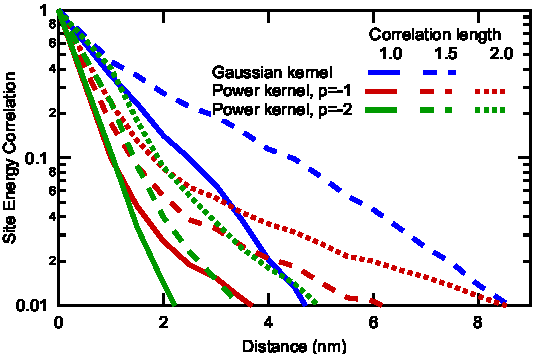
\includegraphics{DOS_correlation_comparison.pdf}
    \caption{Correlated Gaussian disorder model site energy correlation examples showing how the diferent kernel functions cause the correlation to decay as a function of distance.}
    \label{fig:correlation_data}
\end{figure}

\subsubsection{Exponential Disorder Model}

The standard exponential distribution, unlike a Gaussian, is discontinuous at zero and does not contain a high energy tail as would be expected in real materials.
To create a more appropriate overall density of states distribution, while retaining the exponential tail states, a hybrid exponential-Gaussian density of states model is implemented, such that the median state energy remains at zero.
Half of the sites above zero (high energy sites) are assigned using a Gaussian distribution, and the other half of low energy sites below zero are assigned using an exponential distribution.
The Gaussian half is constrained such that its peak is continuous with the maximum of the exponential distribution.
As a result, the overall distribution is defined only by the exponential distribution's Urbach energy ($E_\text{u}$) and the standard deviation of the Gaussian is automatically set to meet the continuity constraint.
Figure \ref{fig:exponential_dos} shows an example of the hybrid exponential-Gaussian density of states distribution compared to the standard Gaussian shape.

\begin{figure}[h]
    \centering
    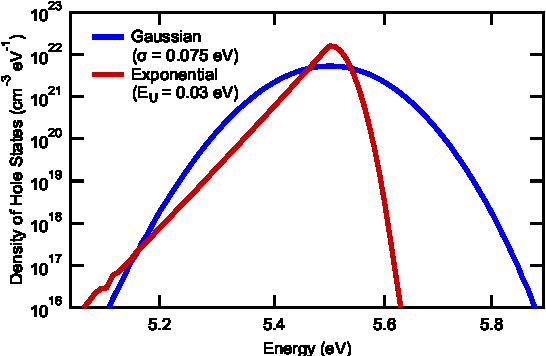
\includegraphics{DOS_shape_comparison.pdf}
    \caption{Density of states distributions for the exponential disorder model compared to the Gaussian disorder model.}
    \label{fig:exponential_dos}
\end{figure}

\subsection{Electrostatic Interaction Parameters}

Electrostatic interactions between polarons are an important factor in determining polaron recombination rates\cite{heiber2016prb} and transport behavior\cite{vanderholst2011prb}.
Users can set the dielectric constant ($\epsilon$), which acts to screen these interactions.
Coulomb interactions are included between each polaron pair as long as their separation distance is less than the Coulomb cutoff radius ($r_{\text{C,cut}}$).
The Coulomb cutoff radius can be explicitly defined in the parameter file or it can be set to dynamically scale with the size of the lattice.
It is not recommended to set the cutoff radius to be larger than half of the smallest dimension in order to prevent double counting interactions with the same polaron across the periodic boundaries.

\subsection{Input Physical Parameter List}

\begin{center}
\begin{tabular}{ c l l }
\hline
 & KMC Algorithm Parameters & \\
 \hline
$r_{\text{recalc}}$ & event recalculation cutoff radius & (nm) \\
\hline
 & Lattice Parameters & \\
\hline
$L$ & lattice length (x-dimension size) & ($a$) \\
$W$ & lattice width (y-dimension size) & ($a$) \\
$H$ & lattice height (z-dimension size) & ($a$) \\
$a$ & lattice unit size & (nm) \\
$T$ & temperature & (K) \\
$V_\text{int}$ & internal voltage & (V) \\
\hline
& Site Parameters & \\
\hline
$E_\text{HOMO}$ & highest occupied molecular orbital energy & (eV) \\
$E_\text{LUMO}$ & lowest unoccupied molecular orbital energy & (eV) \\
$E_\text{U}$ & exponential DOS Urbach energy & (eV) \\
$\epsilon$ & dielectric constant & (unitless) \\
$\sigma$ & Gaussian DOS standard deviation & (eV) \\
\hline
 & Exciton Parameters & \\
 \hline
$E_\text{B}$ & exciton binding energy & (eV) \\
$G$ & singlet exciton generation rate & (cm$^{-3}$ s$^{-1}$) \\
$R_{0,\text{risc}}$ & reverse intersystem crossing rate prefactor & (s$^{-1}$) \\
$R_{0,\text{sxh}}$ & singlet exciton hopping rate prefactor & (nm$^6$ s$^{-1}$) \\
$R_{0,\text{txh}}$ & triplet exciton hopping rate prefactor & (s$^{-1}$) \\
$R_{0,\text{xd}}$ & exciton dissociation rate prefactor & (s$^{-1}$) \\
$R_{0,\text{xxa}}$ & exciton-exciton annihilation rate prefactor & (nm$^{6}$ s$^{-1}$ or s$^{-1}$) \\
$R_{0,\text{xpa}}$ & exciton-polaron annihilation rate prefactor & (nm$^{6}$ s$^{-1}$ or s$^{-1}$) \\ 
$R_{\text{isc}}$ & intersystem crossing rate & (s$^{-1}$) \\
$r_{\text{FRET,cut}}$ & FRET cutoff radius & (nm) \\
$r_{\text{xd,cut}}$ & exciton dissociation cutoff radius & (nm) \\
$\gamma_\text{s}$ & singlet exciton localization parameter & (nm$^{-1}$) \\
$\gamma_\text{t}$ & triplet exciton localization parameter & (nm$^{-1}$) \\
$\Delta E_\text{ST}$ & singlet-triplet splitting energy & (eV) \\
$\tau_\text{sx}$ & singlet exciton lifetime & (s) \\
$\tau_\text{tx}$ & triplet exciton lifetime & (s) \\
\hline
 & Polaron Parameters & \\
 \hline
 $R_{0,\text{ph}}$ & polaron hopping rate prefactor & (s$^{-1}$) \\
$R_{0,\text{pr}}$ & polaron recombination rate prefactor & (s$^{-1}$) \\
$r_{\text{C,cut}}$ & Coulomb cutoff radius & (nm) \\
$r_{\text{ph,cut}}$ & polaron hopping cutoff radius & (nm) \\
$\gamma_\text{p}$ & polaron localization parameter & (nm$^{-1}$) \\
$\lambda$ & reorganization energy & (eV) \\
$\sigma_\text{p}$ & Gaussian polaron delocalization
length & (nm) \\
\end{tabular}
\end{center}

\section{Program Installation}

\subsection{Linux (Ubuntu)}

\begin{enumerate}
\item Install Open MPI:
\begin{minted}{shell}
sudo apt-get -y install -qq openmpi-bin libopenmpi-dev
\end{minted}

\item Download Excimontec source files:
    
To download the entire repository, use
\begin{minted}{shell}
git clone --recurse-submodules https://github.com/MikeHeiber/Excimontec
\end{minted}
By default, this will checkout the latest version on the master branch. 
To then checkout a specific tagged release (like v1.0.0), use
\begin{minted}{shell}
git checkout tags/v1.0.0
\end{minted}
To only download a specific release (like v1.0.0), use 
\begin{minted}{shell}
git clone --recurse-submodules https://github.com/MikeHeiber/Excimontec --branch=v1.0.0
\end{minted}

\item Build and Test Excimontec:

When first using Excimontec on your computer, you should build and run the test suite to make sure everything is working correctly.    
Set the Excimontec directory as the current working directory,
\begin{minted}{shell}
cd Excimontec
\end{minted}
and then use GNU Make to build the test executable.
\begin{minted}{shell}
make test
\end{minted}
Once the build is complete, run the test suite
\begin{minted}{shell}
./test/Excimontec_tests.exe
\end{minted}
If there are no test errors, build the main executable.
\begin{minted}{shell}
make
\end{minted}
If everything builds correctly, you can run a simple test using the default parameters.
\begin{minted}{shell}
mpiexec -n 4 Excimontec.exe parameters_default.txt
\end{minted}

This will execute a simple exciton diffusion simulation test, and when it finishes several output files will be created in the project directory.
You can quickly check the results in the analysis\_summary file with the command.
\begin{minted}{shell}
cat analysis_summary.txt
\end{minted}
The default parameters should produce an exciton diffusion length of approximately 24 nm.

\end{enumerate}

\subsection{Windows 10}

\begin{enumerate}
    \item Install Ubuntu via Windows Subsystem for Linux:
    
    Follow the instructions from
    
    \url{https://docs.microsoft.com/en-us/windows/wsl/install-win10}
    
    \item Follow the Linux installation instructions
\end{enumerate}

\subsection{Windows (older versions)}

\begin{enumerate}

\item Install Microsoft Visual Studio 2019 IDE:
    
Download Microsoft Visual Studio IDE from

\url{https://visualstudio.microsoft.com/}

and make sure to install the C++ development tools.

\item Install Microsoft MPI:

Download the Microsoft MPI files from
    
\url{https://docs.microsoft.com/en-us/message-passing-interface/microsoft-mpi}
    
and then install both MS-MPI and the MS-MPI Software Development Kit.

\item Download (Clone) Excimontec Files:

Open Microsoft Visual Studio 2019 and select "Clone or checkout code".

Enter the repository address,
\url{https://github.com/MikeHeiber/Excimontec}
and then click Clone.

Once cloning is finished, the Excimontec repository will be loaded into the Solution Explorer pane on the left.

\item Load Microsoft Visual Studio Solution:

In the Solution Explorer, open the msvc\textbackslash 2019\textbackslash\ folder and then double click the Excimontec.sln solution file.
Once loaded, the Solution Explorer should show three projects: Excimontec, Excimontec\_tests, gtest.

The solution file is set to build Excimontec for 64 bit systems, but this can be changed to 32 bit by changing the build platform using the drop down box in the toolbar at the top.

\item Build and Test Excimontec:

When first using Excimontec on your computer, you should build and run the test suite to make sure everything is working correctly.
To do this, build the gtest project first by right-clicking gtest in the Solution Explorer and selecting Build.

Once the gtest build is complete, right click the Excimontec\_test project in the Solution Explorer and select Build. 

Once the Excimontec\_test build is complete, make it the active project by right clicking the Excimontec\_test project and selecting Set as Startup Project, and then press Cntrl+F5 to run the test suite without the debugger.

If there are no test errors, build the main executable by right-clicking on Excimontec in the Solution Explorer and selecting Build.

If it builds correctly, you can run a simple test using the default parameters.
First, open the command prompt and change the working directory to the Excimontec build directory.

\begin{minted}{shell}
cd %HOMEDRIVE%%HOMEPATH%\Source\Repos\Excimontec\msvc\2019\x64-Release
\end{minted}

Then run Excimontec with the default parameters.
\begin{minted}{shell}
mpiexec -n 4 Excimontec.exe ..\..\..\parameters_default.txt
\end{minted}

This will execute a simple exciton diffusion simulation test, and when it finishes several output files will be created in the build directory.
You can quickly check the results in the analysis\_summary file with the command.
\begin{minted}{shell}
type analysis_summary.txt
\end{minted}
The default parameters should produce an exciton diffusion length of approximately 24 nm.


\end{enumerate}

\bibliography{references}

\end{document}
